\documentclass[11pt,a4paper]{article}

\usepackage[a4paper,margin=2.2cm]{geometry}
\usepackage[utf8]{inputenc}
\usepackage[T1]{fontenc}
\usepackage{lmodern}
\usepackage{xcolor}
\usepackage{tikz}
\usetikzlibrary{arrows.meta, positioning, fit, backgrounds}
\usepackage{tcolorbox}
\tcbuselibrary{skins,breakable}
\usepackage{enumitem}
\usepackage{titlesec}
\usepackage{fancyhdr}
\usepackage{hyperref}
\usepackage{array}
\usepackage{tabularx}
\usepackage{colortbl}

% ---------- Palette ----------
\definecolor{ykgreen}{HTML}{1F4D3A}
\definecolor{ykgreenlight}{HTML}{E8F0EC}
\definecolor{ykamber}{HTML}{B5732A}
\definecolor{ykred}{HTML}{A63D3D}
\definecolor{ykblue}{HTML}{2E5C8A}
\definecolor{ykgray}{HTML}{5A6B65}
\definecolor{ykline}{HTML}{D8E0DC}

\hypersetup{colorlinks=true, linkcolor=ykgreen, urlcolor=ykamber}

\titleformat{\section}
  {\normalfont\Large\bfseries\color{ykgreen}}
  {\textcolor{ykamber}{\thesection}}{0.6em}{}
\titlespacing*{\section}{0pt}{1.3em}{0.7em}

\titleformat{\subsection}
  {\normalfont\large\bfseries\color{ykgreen}}
  {}{0em}{}
\titlespacing*{\subsection}{0pt}{1em}{0.4em}

\pagestyle{fancy}
\fancyhf{}
\renewcommand{\headrulewidth}{0pt}
\fancyfoot[C]{\small\color{ykgray} YANFL\`E \textperiodcentered\ Documentation d'architecture \textperiodcentered\ \thepage}

\newtcolorbox{notecard}{
  colback=ykgreenlight, colframe=ykgreen, boxrule=0.6pt, arc=1pt,
  left=10pt, right=10pt, top=8pt, bottom=8pt
}

\setlength{\parindent}{0pt}
\setlength{\parskip}{0.5em}

\begin{document}

% ============ PAGE DE GARDE ============
\begin{tcolorbox}[colback=ykgreen, colframe=ykgreen, arc=2pt,
  left=18pt, right=18pt, top=16pt, bottom=16pt]
  {\color{white}\fontsize{30}{34}\selectfont\bfseries YANFL\`E}\\[4pt]
  {\color{ykgreenlight}\large Documentation d'architecture technique}
  \vspace{6pt}

  {\color{ykgreenlight}
  YANFL\`E fait passer la vid\'eosurveillance d'un r\^ole de t\'emoin --- qui ne sert qu'\`a constater
  un acte apr\`es coup --- \`a un r\^ole de \textbf{vigie} : un syst\`eme qui comprend ce qu'il observe
  sur un r\'eseau de cam\'eras, pour aider \`a \textbf{pr\'evenir un danger avant qu'il ne se
  produise}, plut\^ot que de simplement le filmer. Ce document d\'ecrit l'architecture technique du
  MVP qui met en \oe uvre une premi\`ere partie de cette vision, ex\'ecut\'e localement sur un serveur
  \'equip\'e GPU.
  }
\end{tcolorbox}

\vspace{10pt}

\renewcommand{\contentsname}{Table des mati\`eres}
\tableofcontents

% ============ 1. VUE D'ENSEMBLE ============
\section{Vue d'ensemble}

YANFL\`E transforme des cam\'eras ordinaires (t\'el\'ephones ou PC sur le m\^eme r\'eseau) en un
r\'eseau de vid\'eosurveillance intelligent. Chaque image captur\'ee traverse une \textbf{cha\^ine de
9 mod\`eles de d\'etection} plus un module de reconnaissance faciale, et le tout est r\'esum\'e par un
narrateur factuel. Le syst\`eme est organis\'e autour de \textbf{cinq interfaces web}, chacune pour un
usage pr\'ecis, et d'un \textbf{serveur central} qui fait tourner l'intelligence artificielle.

\subsection*{Ce document par rapport au dossier de pitch}

Le dossier de pr\'esentation initial (\emph{YANFL\`E --- Orange Summer Challenge 2026}) posait une
\textbf{vision en quatre principes}, \`a un stade o\`u \emph{"la conception, l'entra\^inement du
mod\`ele et les tests rest[ai]ent enti\`erement \`a faire"}. Ce document d\'ecrit l'architecture du
\textbf{MVP} qui en a \'et\'e tir\'e depuis : une preuve de concept fonctionnelle, mais partielle, et
qui s'\'ecarte par endroits --- volontairement --- de la vision initiale. Le tableau ci-dessous fait
le point, principe par principe.

\begin{center}
\renewcommand{\arraystretch}{1.4}
\begin{tabularx}{\linewidth}{@{}p{4.3cm}X@{}}
\hline
\textbf{Principe du pitch} & \textbf{\'Etat dans ce MVP} \\
\hline
1. Observer le comportement, pas l'identit\'e &
\textbf{\'Ecart assum\'e.} Le MVP ajoute une reconnaissance faciale (Le Physionomiste, \S\ref{sec:visages})
avec gestion d'autorisations par lieu --- l'inverse du principe initial. Ce choix a \'et\'e fait en
cours de route pour permettre la d\'etection de pr\'esence non autoris\'ee, plus concr\`ete \`a
d\'emontrer qu'une simple analyse de posture. \\
2. Reconna\^itre les signaux qui pr\'ec\`edent un acte &
\textbf{Partiellement couvert.} Le Secouriste rep\`ere une chute d\'ej\`a survenue (r\`egle
g\'eom\'etrique sur le squelette). Aucun mod\`ele ne d\'etecte encore un comportement
\emph{pr\'ecurseur} (r\^odage prolong\'e, posture d'agression avant le geste) --- c'est la brique la
plus proche de la promesse initiale du projet, et elle reste \`a construire. \\
3. Alerter un humain, ne jamais d\'ecider seul &
\textbf{Respect\'e.} Tous les r\'esultats (\texttt{/vision}, \texttt{/bat}) sont pr\'esent\'es \`a un
superviseur humain ; le syst\`eme ne d\'eclenche aucune action automatique, il signale. \\
4. Adapter la r\'eponse \`a la gravit\'e (appel vocal automatis\'e) &
\textbf{Non impl\'ement\'e.} La narration et les alertes visuelles (dangers, pr\'esences non
autoris\'ees) existent, mais aucune escalade par appel t\'el\'ephonique automatis\'e n'a \'et\'e
d\'evelopp\'ee. \\
\hline
\end{tabularx}
\end{center}

\subsection*{Les cinq interfaces}

\begin{center}
\renewcommand{\arraystretch}{1.4}
\begin{tabularx}{\linewidth}{@{}lX@{}}
\hline
\textbf{Route} & \textbf{R\^ole} \\
\hline
\texttt{/admin} & Cr\'eer des \textbf{b\^atiments}, des \textbf{points} (portail, bureau, ...) et des
\textbf{cam\'eras} (chacune avec un code unique g\'en\'er\'e automatiquement). \\
\texttt{/cam} & Interface qu'un t\'el\'ephone ou PC ouvre pour \textbf{devenir une cam\'era} du r\'eseau :
il entre le code, puis d\'emarre/arr\^ete l'envoi de son flux. \\
\texttt{/vision} & Vue de \textbf{supervision globale} : toutes les cam\'eras de tous les b\^atiments,
en direct, group\'ees par b\^atiment. \\
\texttt{/bat} & Vue de supervision \textbf{scop\'ee \`a un seul b\^atiment} (via son propre code) : cam\'eras
en direct, narration unique combin\'ee, et gestion des personnes/autorisations. \\
\texttt{/bat/chat} & Assistant conversationnel : poser des questions en langage naturel sur l'\'etat
r\'eel d'un b\^atiment. \\
\hline
\end{tabularx}
\end{center}

\subsection*{Sch\'ema g\'en\'eral}

\begin{center}
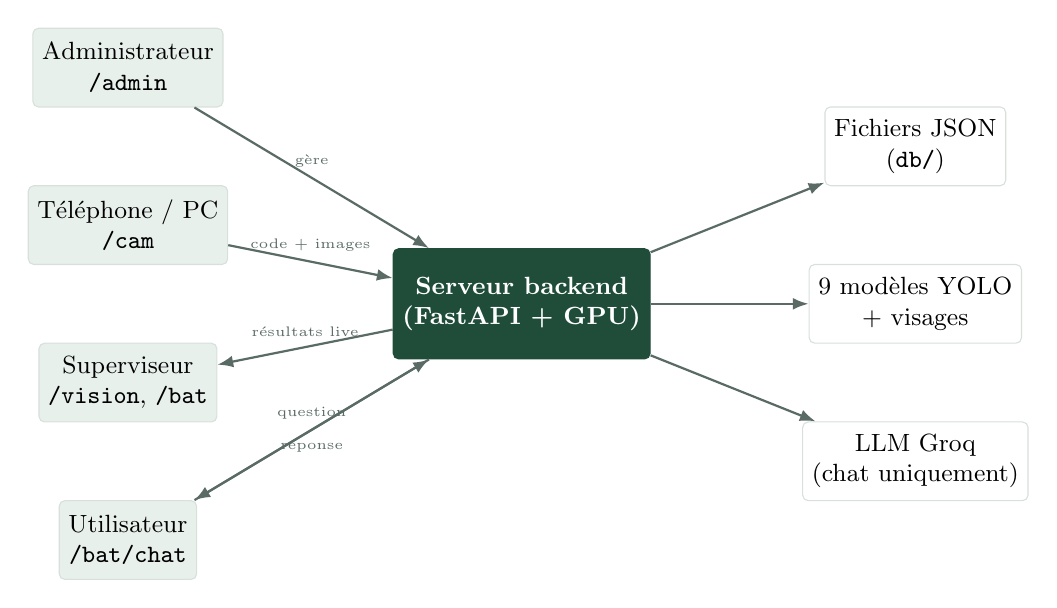
\begin{tikzpicture}[
  box/.style={draw=ykline, fill=ykgreenlight, rounded corners=2pt, minimum height=1cm, align=center, font=\small},
  server/.style={draw=ykgreen, fill=ykgreen, text=white, rounded corners=2pt, minimum height=1.4cm, align=center, font=\small\bfseries},
  arr/.style={-{Latex[length=2mm]}, ykgray, thick}
]
  \node[box] (admin) at (0,4) {Administrateur\\\texttt{/admin}};
  \node[box] (cam) at (0,2) {T\'el\'ephone / PC\\\texttt{/cam}};
  \node[box] (vision) at (0,0) {Superviseur\\\texttt{/vision}, \texttt{/bat}};
  \node[box] (chat) at (0,-2) {Utilisateur\\\texttt{/bat/chat}};

  \node[server] (backend) at (5,1) {Serveur backend\\(FastAPI + GPU)};

  \node[box, fill=white] (db) at (10,3) {Fichiers JSON\\(\texttt{db/})};
  \node[box, fill=white] (models) at (10,1) {9 mod\`eles YOLO\\+ visages};
  \node[box, fill=white] (llm) at (10,-1) {LLM Groq\\(chat uniquement)};

  \draw[arr] (admin) -- node[above,font=\tiny] {g\`ere} (backend);
  \draw[arr] (cam) -- node[above,font=\tiny] {code + images} (backend);
  \draw[arr] (backend) -- node[above,font=\tiny] {r\'esultats live} (vision);
  \draw[arr] (chat) -- node[above,font=\tiny] {question} (backend);
  \draw[arr] (backend) -- node[below,font=\tiny] {r\'eponse} (chat);

  \draw[arr] (backend) -- (db);
  \draw[arr] (backend) -- (models);
  \draw[arr] (backend) -- (llm);
\end{tikzpicture}
\end{center}

% ============ 2. LA CHAINE D'ANALYSE ============
\section{La cha\^ine d'analyse}

Chaque image envoy\'ee par une cam\'era (via \texttt{/cam}) ou par la page de d\'emonstration passe par
la m\^eme cha\^ine, ex\'ecut\'ee enti\`erement sur le serveur.

\begin{center}
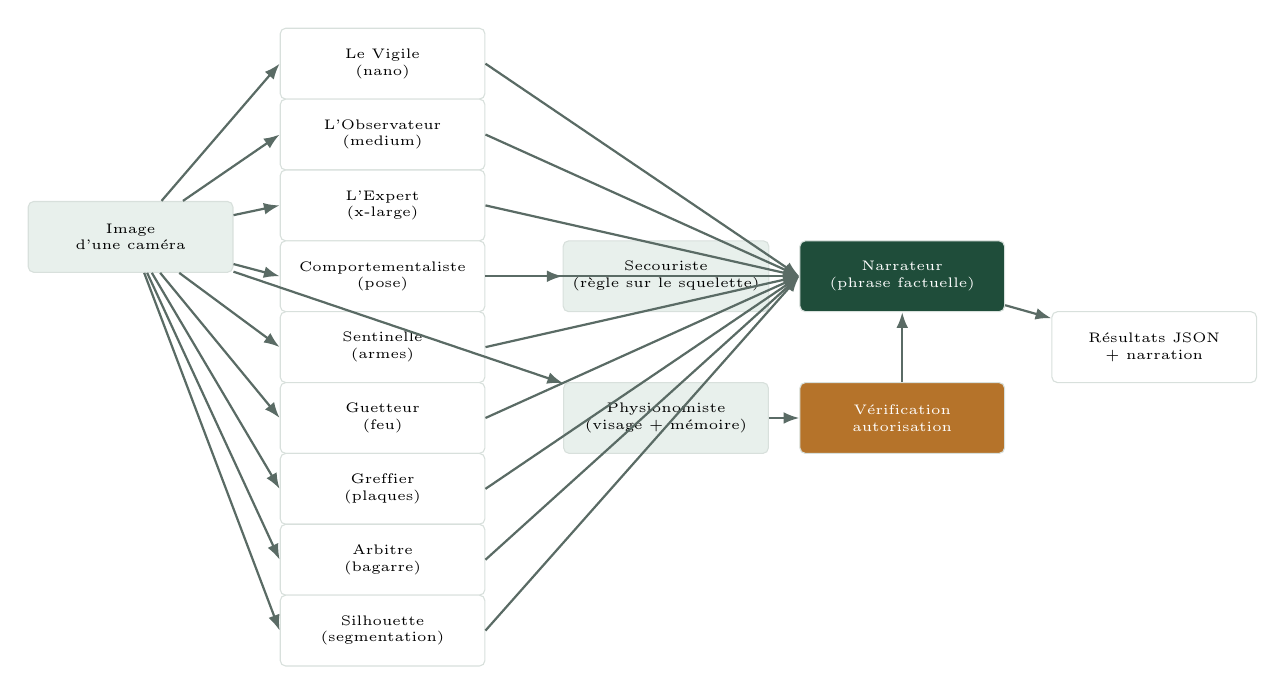
\begin{tikzpicture}[
  flowbox/.style={draw=ykline, fill=white, rounded corners=2pt, minimum width=2.6cm, minimum height=0.9cm, align=center, font=\tiny},
  arr/.style={-{Latex[length=2mm]}, ykgray, thick}
]
  \node[flowbox, fill=ykgreenlight] (img) at (0,0) {Image\\d'une cam\'era};

  \node[flowbox] (nano) at (3.2,2.2) {Le Vigile\\(nano)};
  \node[flowbox] (medium) at (3.2,1.3) {L'Observateur\\(medium)};
  \node[flowbox] (xlarge) at (3.2,0.4) {L'Expert\\(x-large)};
  \node[flowbox] (pose) at (3.2,-0.5) {Comportementaliste\\(pose)};
  \node[flowbox] (threat) at (3.2,-1.4) {Sentinelle\\(armes)};
  \node[flowbox] (fire) at (3.2,-2.3) {Guetteur\\(feu)};
  \node[flowbox] (plate) at (3.2,-3.2) {Greffier\\(plaques)};
  \node[flowbox] (fight) at (3.2,-4.1) {Arbitre\\(bagarre)};
  \node[flowbox] (seg) at (3.2,-5.0) {Silhouette\\(segmentation)};

  \node[flowbox, fill=ykgreenlight] (fall) at (6.8,-0.5) {Secouriste\\(r\`egle sur le squelette)};
  \node[flowbox, fill=ykgreenlight] (face) at (6.8,-2.3) {Physionomiste\\(visage + m\'emoire)};

  \node[flowbox, fill=ykamber, text=white] (auth) at (9.8,-2.3) {V\'erification\\autorisation};

  \node[flowbox, fill=ykgreen, text=white] (narr) at (9.8,-0.5) {Narrateur\\(phrase factuelle)};

  \node[flowbox, fill=white] (out) at (13,-1.4) {R\'esultats JSON\\+ narration};

  \foreach \m in {nano,medium,xlarge,pose,threat,fire,plate,fight,seg}
    \draw[arr] (img) -- (\m.west);

  \draw[arr] (pose) -- (fall);
  \draw[arr] (img) -- (face);
  \draw[arr] (face) -- (auth);
  \foreach \m in {nano,medium,xlarge,pose,threat,fire,plate,fight,seg,fall}
    \draw[arr] (\m.east) -- (narr.west);
  \draw[arr] (auth) -- (narr);
  \draw[arr] (narr) -- (out);
\end{tikzpicture}
\end{center}

\subsection*{D\'etail des 9 mod\`eles + 2 modules d\'eriv\'es}

\begin{center}
\renewcommand{\arraystretch}{1.3}
\begin{tabularx}{\linewidth}{@{}lX@{}}
\hline
\textbf{R\^ole} & \textbf{Ce qu'il fait} \\
\hline
\textbf{Le Vigile} & D\'etection rapide (mod\`ele nano), premier coup d'\oe il. \\
\textbf{L'Observateur} & D\'etection interm\'ediaire (medium), plus fiable. \\
\textbf{L'Expert} & D\'etection la plus pr\'ecise (x-large), r\'ef\'erence pour la narration. \\
\textbf{Le Comportementaliste} & Squelette (17 points cl\'es) + suivi de chaque personne dans le temps (\texttt{track\_id}). \\
\textbf{La Sentinelle} & D\'etection d'armes/objets dangereux (mod\`ele communautaire, seuil de confiance relev\'e). \\
\textbf{Le Guetteur} & D\'etection de feu et de fum\'ee. \\
\textbf{Le Greffier} & D\'etection de plaques d'immatriculation. \\
\textbf{L'Arbitre} & D\'etection de bagarre / comportement violent. \\
\textbf{Le Silhouette} & Segmentation (contour exact au pixel). \\
\textbf{Le Secouriste} & \emph{Pas un mod\`ele} : r\`egle g\'eom\'etrique sur le squelette (torse \`a plat + bo\^ite
plus large que haute) pour rep\'erer une chute. \\
\textbf{Le Physionomiste} & Reconnaissance faciale (MTCNN + InceptionResnetV1) avec m\'emoire persistante \`a deux
niveaux (voir \S\ref{sec:visages}). \\
\hline
\end{tabularx}
\end{center}

\begin{notecard}
\textbf{Isolation par cam\'era} : chaque cam\'era poss\`ede son propre jeu des 9 mod\`eles, charg\'e \`a la
demande. Cela \'evite que le suivi temporel (\texttt{track\_id}) d'une cam\'era ne se m\'elange avec celui
d'une autre. La reconnaissance faciale, elle, reste \textbf{globale} : une personne reconnue l'est sur
n'importe quelle cam\'era du r\'eseau.
\end{notecard}

% ============ 3. RECONNAISSANCE FACIALE ============
\section{Reconnaissance faciale \`a deux m\'emoires}
\label{sec:visages}

Pour \'eviter qu'un visage crois\'e une seule fois ne devienne imm\'ediatement une "personne", le
syst\`eme utilise deux bases distinctes :

\begin{center}
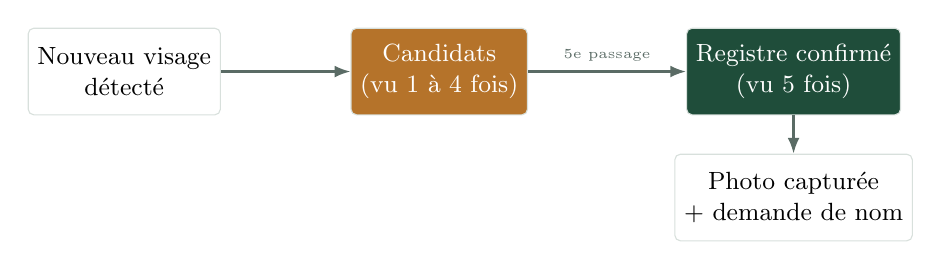
\begin{tikzpicture}[
  box/.style={draw=ykline, fill=white, rounded corners=2pt, minimum height=1.1cm, align=center, font=\small},
  arr/.style={-{Latex[length=2mm]}, ykgray, thick}
]
  \node[box] (new) at (0,0) {Nouveau visage\\d\'etect\'e};
  \node[box, fill=ykamber, text=white] (cand) at (4,0) {Candidats\\(vu 1 \`a 4 fois)};
  \node[box, fill=ykgreen, text=white] (reg) at (8.5,0) {Registre confirm\'e\\(vu 5 fois)};
  \node[box] (photo) at (8.5,-1.6) {Photo captur\'ee\\+ demande de nom};

  \draw[arr] (new) -- (cand);
  \draw[arr] (cand) -- node[above,font=\tiny]{5e passage} (reg);
  \draw[arr] (reg) -- (photo);
\end{tikzpicture}
\end{center}

\begin{itemize}[leftmargin=1.2em, itemsep=3pt]
  \item \textbf{Seuil de confiance visage} : 92\% minimum (\'evite les faux positifs sur des motifs/ombres).
  \item \textbf{Seuil de confirmation} : 5 apparitions similaires avant promotion.
  \item \`A la promotion, une \textbf{photo} est sauvegard\'ee et l'interface demande un nom (ou permet de
  marquer \emph{"Inconnu N"}, num\'erot\'e automatiquement).
  \item Un nom peut \^etre modifi\'e \`a tout moment depuis \texttt{/bat} $\rightarrow$ \emph{G\'erer les personnes}.
\end{itemize}

\subsection*{Autorisations par point}

Chaque personne confirm\'ee peut \^etre \textbf{autoris\'ee} sur une liste de points (ex : "Portail",
"Bureau 3") propres \`a un b\^atiment. Si elle est reconnue sur une cam\'era associ\'ee \`a un point
o\`u elle n'est \textbf{pas} autoris\'ee, le syst\`eme l'indique clairement
(\textbf{présence non autorisée}) dans l'affichage et dans la narration. Une personne marqu\'ee
\emph{"Inconnu"} n'a par d\'efinition aucune autorisation nulle part.

% ============ 4. NARRATION ============
\section{Narration factuelle (sans IA g\'en\'erative)}

Un point important de conception : la description en langage naturel de ce qui se passe
(\emph{"D\'etect\'e : 1 bus, 4 personnes."}) n'est \textbf{pas} g\'en\'er\'ee par un grand mod\`ele de
langage. Une premi\`ere version utilisait un LLM (Groq / Llama) pour un style plus "vivant", mais ce
dernier inventait parfois des d\'etails absents des donn\'ees (noms, objets, actions). Le narrateur a
donc \'et\'e r\'e\'ecrit en \textbf{g\'en\'eration d\'eterministe} : une phrase construite directement \`a
partir des faits d\'etect\'es, mot pour mot, sans aucune part de cr\'eativit\'e — donc sans risque
d'invention.

\begin{notecard}
Le LLM (Groq, mod\`ele \texttt{llama-3.1-8b-instant}) n'est utilis\'e que dans \texttt{/bat/chat}, o\`u il
r\'epond \`a des questions libres \textbf{uniquement} \`a partir des donn\'ees r\'eelles fournies en
contexte, avec instruction stricte de r\'epondre "je ne sais pas" plut\^ot que d'inventer.
\end{notecard}

% ============ 5. MODELE DE DONNEES ============
\section{Mod\`ele de donn\'ees}

\begin{center}
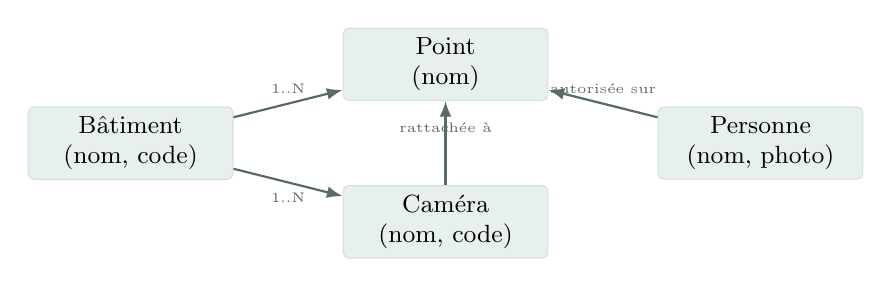
\begin{tikzpicture}[
  ent/.style={draw=ykline, fill=ykgreenlight, rounded corners=2pt, minimum width=2.6cm, minimum height=0.9cm, align=center, font=\small},
  arr/.style={-{Latex[length=2mm]}, ykgray, thick}
]
  \node[ent] (bat) at (0,0) {B\^atiment\\(nom, code)};
  \node[ent] (point) at (4,1) {Point\\(nom)};
  \node[ent] (cam) at (4,-1) {Cam\'era\\(nom, code)};
  \node[ent] (pers) at (8,0) {Personne\\(nom, photo)};

  \draw[arr] (bat) -- node[above,font=\tiny]{1..N} (point);
  \draw[arr] (bat) -- node[below,font=\tiny]{1..N} (cam);
  \draw[arr] (cam) -- node[above,font=\tiny]{rattach\'ee \`a} (point);
  \draw[arr] (pers) -- node[above,font=\tiny]{autoris\'ee sur} (point);
\end{tikzpicture}
\end{center}

Chaque \textbf{b\^atiment} et chaque \textbf{cam\'era} poss\`ede un code unique g\'en\'er\'e
automatiquement (ex : \texttt{A1B2-C3D4}), qui sert de moyen d'acc\`es simple (pas de mot de passe) \`a
\texttt{/cam} et \texttt{/bat}.

% ============ 6. STOCKAGE ============
\section{Stockage}

Aucune base de donn\'ees externe : tout est enregistr\'e en fichiers JSON dans \texttt{db/}, pour
rester simple et inspectable directement.

\begin{center}
\renewcommand{\arraystretch}{1.3}
\begin{tabularx}{\linewidth}{@{}lX@{}}
\hline
\textbf{Fichier / dossier} & \textbf{Contenu} \\
\hline
\texttt{buildings.json} & B\^atiments, points, cam\'eras (avec leurs codes). \\
\texttt{faces\_candidates.json} & Visages en observation (pas encore confirm\'es). \\
\texttt{faces\_registry.json} & Personnes confirm\'ees : nom, photo, autorisations. \\
\texttt{faces/} & Photos des personnes confirm\'ees. \\
\texttt{cameras/<id>/detections\_*.jsonl} & Historique des d\'etections, par cam\'era et par jour. \\
\texttt{cameras/<id>/narration\_*.jsonl} & Historique des phrases de narration, s\'epar\'e des d\'etections. \\
\hline
\end{tabularx}
\end{center}

% ============ 7. SECURITE ============
\section{S\'ecurit\'e}

\begin{itemize}[leftmargin=1.2em, itemsep=3pt]
  \item Le serveur tourne en \textbf{HTTPS} (certificat auto-sign\'e) : indispensable pour que les
  navigateurs mobiles autorisent l'acc\`es \`a la cam\'era en dehors de \texttt{localhost}.
  \item Acc\`es par \textbf{code unique} pour chaque cam\'era et chaque b\^atiment — pas de compte
  utilisateur \`a ce stade (adapt\'e \`a un usage interne sur r\'eseau local).
  \item Les donn\'ees biom\'etriques (embeddings de visage) restent \textbf{stock\'ees localement},
  jamais transmises \`a un service externe.
\end{itemize}

% ============ 8. LIMITES CONNUES ============
\section{Limites connues et pistes}

\subsection*{Pour se rapprocher de la vision initiale}

Par ordre de priorit\'e si l'objectif est de revenir vers la promesse du dossier de pitch
(comparatif en \S1, \emph{"Ce document par rapport au dossier de pitch"}) :

\begin{enumerate}[leftmargin=1.2em, itemsep=3pt]
  \item \textbf{D\'etection de signaux pr\'ecurseurs} (principe 2) : entra\^iner ou int\'egrer un
  mod\`ele qui reconna\^it un r\^odage prolong\'e ou une posture d'agression \`a partir du squelette
  d\'ej\`a extrait par Le Comportementaliste, plut\^ot que de se limiter \`a la chute (d\'ej\`a
  survenue).
  \item \textbf{Escalade par appel vocal} (principe 4) : brancher un service de t\'el\'ephonie
  automatis\'ee (ex. SIP + voix de synth\`ese) sur les alertes critiques d\'ej\`a d\'etect\'ees
  (armes, feu, bagarre), avec confirmation requise du responsable.
  \item \textbf{Reconnaissance faciale} (principe 1) : si l'\'ecart reste probl\'ematique pour le jury
  ou pour des raisons de conformit\'e, le module Physionomiste peut \^etre d\'esactiv\'e sans toucher
  au reste de la cha\^ine --- il est ind\'ependant des 9 autres mod\`eles.
\end{enumerate}

\subsection*{Limites techniques du MVP actuel}

\begin{itemize}[leftmargin=1.2em, itemsep=3pt]
  \item Les mod\`eles communautaires (Sentinelle, Greffier, Arbitre) ont une pr\'ecision plus faible que
  les mod\`eles officiels YOLO11 — seuils de confiance relev\'es pour limiter les faux positifs, \`a
  surveiller en usage r\'eel.
  \item La reconnaissance faciale peut cr\'eer plusieurs identifiants pour la m\^eme personne si
  l'\'eclairage/l'angle varie beaucoup (embeddings trop diff\'erents pour matcher) — fusion manuelle
  possible via suppression dans \emph{G\'erer les personnes}.
  \item Le narrateur factuel est fiable mais moins "vivant" qu'une g\'en\'eration libre — compromis
  assum\'e pour \'eliminer tout risque d'invention.
  \item Le chat (\texttt{/bat/chat}) d\'epend d'une cl\'e API Groq externe — \`a surveiller en cas de
  changement de disponibilit\'e du service.
\end{itemize}

\vspace{1em}
\begin{center}
\small\color{ykgray}\textsc{YANFL\`E --- Tech Impact --- Orange Summer Challenge 2026}
\end{center}

\end{document}
